\documentclass[12pt]{report}
\usepackage{graphicx}
\usepackage{titling}
\usepackage{fancyhdr}
\usepackage[latin1]{inputenc}
\usepackage{enumerate}
\usepackage{float}
\usepackage{latexsym}
\usepackage{amssymb}
\usepackage{amsthm}
\usepackage{amsfonts}
\usepackage{amsmath}
\usepackage[labelfont=bf]{caption}
\usepackage[usenames,dvipsnames,svgnames,table]{xcolor}
\usepackage{listings}
\parindent=0pt
\frenchspacing

\pagestyle{fancy}

\newcommand{\pctlrepeat}[1]{{\buildrel{#1}\over\curvearrowleft}}

\fancyhead[L]{\slshape\footnotesize December 3, 2013\\\textsc{02246 Model Checking}}
\fancyhead[R]{\slshape\footnotesize \textsc{Andreas Kjeldsen (s092638)}\\\textsc{Morten Eskesen (s133304)}}
\fancyfoot[C]{\thepage}

\lstdefinestyle{logoutput}{
	backgroundcolor=\color[RGB]{248,248,248},
	tabsize=1,
	captionpos=b
  	belowcaptionskip=1\baselineskip,
  	breaklines=true,
  	frame=single,
	language={},
  	basicstyle=\footnotesize\ttfamily\color{Black}
}

\lstdefinestyle{prismmodel}{
	tabsize=1,
	captionpos=b,
  	belowcaptionskip=1\baselineskip,
  	breaklines=true,
  	frame=single,
	frameround=tttt,
  	language={},
  	numbers=left,
  	numbersep=5pt,
  	numberstyle=\tiny\ttfamily\color{Black},
  	basicstyle=\footnotesize\ttfamily\color{Black},
  	keywordstyle=\bfseries\color{Black},
	morekeywords={module, endmodule, label, init, mdp }, 
	otherkeywords={=, :, [, ], |},
	identifierstyle={\color{red}\let\textcolor\textcolordummy},
	morestring=[b][\color{red}\bfseries]",
	commentstyle=\color{Green},
	moredelim=[s][\color{DarkOrchid}\ttfamily]{[}{]},
	literate=%
		*{0}{{{\color{blue}0}}}1
	    {1}{{{\color{blue}1}}}1
	    {2}{{{\color{blue}2}}}1
	    {3}{{{\color{blue}3}}}1
	    {4}{{{\color{blue}4}}}1
	    {5}{{{\color{blue}5}}}1
	    {6}{{{\color{blue}6}}}1
	    {7}{{{\color{blue}7}}}1
	    {8}{{{\color{blue}8}}}1
	    {9}{{{\color{blue}9}}}1
}

\newcommand{\tab}{\hspace*{2em}}
\newcommand{\HRule}{\rule{\linewidth}{0.5mm}}

\begin{document}

\begin{titlepage}
\begin{center}


\includegraphics[scale=2.0]{../GFX/dtu_logo.pdf}\\[1cm]

\textsc{\LARGE Technical University of Denmark}\\[1.5cm]

\textsc{\Large 02246 Model Checking}\\[0.5cm]


% Title
\HRule \\[0.4cm]
{\huge \bfseries Mandatory Assignment\\Part 2: Stochastic Modelling and Verification in Discrete Time}\\[0.1cm]
\HRule \\[1.5cm]

% Author and supervisor
\large
\emph{Authors:}
\\[10pt]
Andreas Hallberg \textsc{Kjeldsen}\\
\emph{s092638@student.dtu.dk}
\\[10pt]
Morten Chabert \textsc{Eskesen}\\
\emph{s133304@student.dtu.dk}

\vfill

% Bottom of the page
{\large December 3, 2013}

\end{center}
\end{titlepage}

\chapter*{Introductory notes}
This report has been written by the both of us. All parts have been worked on together and therefore our responsibility for each assignment is equal.
\chapter*{Part A: Introductory Problems}
\section*{A1) Practical Problems}

\subsection*{A1.1}
In this problem we will ad probabilities to the FCFS scheduler from the previous assignment, so that we construct a discrete time Markov chain.

\subsubsection*{A1.1a) Non-determinism}
Currently in the FCFS scheduler there are sources of non-determinism. Some of the sources are the create commands in $client_1$ and $client_2$ because there are 5 different create commands with the same guard only the update distinguishes the commands. These sources are due to local non-determinism between the commands in the modules. The other source of non-determinism is due to concurrent execution of the modules in FCFS. The shifting command in the Scheduler module is a result of non-determinism because it can happen independently of what the other modules are doing.

\subsubsection*{A1.1b) Resolve local non-determinism}
In order to resolve the local non-determinism we have to modify the modules to include probabilistic commands. Since the distribution of the probabilities should be uniform the new create command will look like the following:
\begin{lstlisting}[style=prismmodel]
[create1] state1=0 -> 0.2 :(state1'=1) & (task1'=1) +
                      0.2 :(state1'=1) & (task1'=2) +
                      0.2 :(state1'=1) & (task1'=3) +
                      0.2 :(state1'=1) & (task1'=4) + 
                      0.2 :(state1'=1) & (task1'=5);
\end{lstlisting}

\subsubsection*{A1.1c) From MDP to DTMC}
The FCFS file has been changed to have the extension .pm and the first line of the model is 'dtmc' which tells PRISM that the file describes a Discrete Time Markov Chain. Building the model causes no errors and tells us that we now have 83 reachable states in the model. Which was the same as before because PRISM resolves the local non-determinism by using a uniform distribution. If there are 5 possibilities it will choose each with probability $\frac{1}{5}$.

\subsubsection*{A1.1d) From non-deterministic to probabilistic}
As explained earlier the shifting command in the Scheduler module causes some non-determinism. This non-determinism we have due to the concurrent execution of the modules is still there. If there were commands in the other commands in the modules that could happen independently of what the Scheduler module was doing all of these commands would happen with equal probability. Since there are no other commands specified that way the command in the Scheduler module happens with probability 1 when possible. PRISM enforces this.

\subsubsection*{A1.1e) Verify some PCTL formula}
In order to make sure that a job will almost certainly complete we specify the following PRISM properties - one for each client.
\begin{center}
$(task_1 > 0) \Rightarrow \mathbb{P}_{\geq 1}(\diamondsuit(task_1 = 0))$\\
$(task_2 > 0) \Rightarrow \mathbb{P}_{\geq 1}(\diamondsuit(task_2 = 0))$
\end{center}
These properties have been verified by PRISM so we now know that a created job will almost certainly complete in this model.

\subsection*{A1.2}
This section is about using PRISM to compute numerical properties of the FCFS model.

\subsubsection*{A1.2a) Computing the steady state distribution}
If we calculate the steady state distribution of the model we can find the probability of having no jobs in the scheduler. We use PRISM to calculate the steady state distribution and it gives us the probability of being in each of the reachable states. Only one state has no jobs in the scheduler which is the initial:
\begin{lstlisting}[style=logoutput]
0:(0,0,0,0,0,0)=0.016145825133811565
\end{lstlisting}
The probability of having no jobs in the scheduler is therefore 0.0161.

\subsubsection*{A1.2b) Calculating the expected length of a job for $client_1$}
We want to calculate the expected length of a job for $client_1$ by looking at the steady state probabilities. In order to do this computation manually we first have to sum the probabilities of the states where $client_1$ has a job of length $i$, $0 \leq i \leq 5$. These states are states 12--82.
\begin{center}
Probability: 0.75
\end{center}

$$\frac{0 \cdot 0.0911 + 1 \cdot 0.1675 + 2 \cdot 0.1506 + 3 \cdot 0.1331 + 4 \cdot 0.1142 + 5 \cdot 0.0935}{0.75} = 2.39$$
The expected length of a job for $client_1$ is 2.39.
We want to calculate the expected length of a job for $client_1$ by looking at the steady state probabilities. In order to do this computation manually we first have to sum the probabilities of the states where $client_1$ has a job of length $i$, $0 \leq i \leq 5$. These states are states 12--82.

\subsubsection*{A1.2c) Calculating the transient distribution}
We want to know what the probability of $client_1$ not having a job at time $t = 10$ so we calculate the transient distribution of the model at time $t = 10$. When we do this PRISM will output the probability for being in each state at this time and we sum the probabilities of being in states where $client_1$ does not have a job. States where $client_1$ does not have a job are states 0--11. We sum the probability of being in these states and get:
\begin{center}
Probability: 0.2574
\end{center}

\subsubsection*{A1.2d) Showing probability as a graph}
We have to plot a graph of the probability that $client_1$ does not have a job against time $t$, for $0 \leq t \leq 10$. We therefore calculate the transient distribution of the model for time $t$. We sum the probabilities of the states where $client_1$ does not have a job. We can then plot the graph of the probability.\\
\begin{figure}[H]
	\centering
	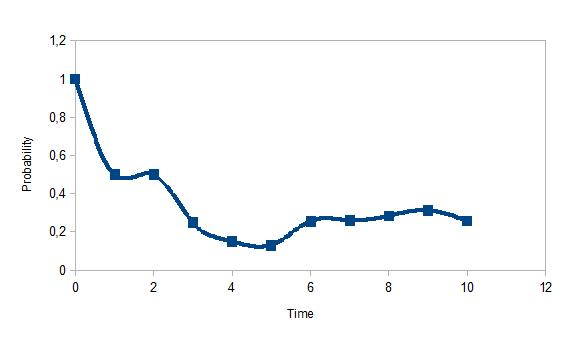
\includegraphics[scale=0.9]{../GFX/A1-2d.png}
	\caption{The graph for for A1.2d}
\end{figure}
The graph starts a probability 1 because in the initial state there is no jobs in the scheduler. Then the probability falls to 0.5 because there is an equal probability of $client_1$ and $client_2$ creating a job. After that the probability is between 0.15 and 0.30 which is quite low because each client can always have one job in the scheduler therefore there is a higher probability of the clients having a job in the scheduler.

\subsection*{A1.3}
This part is about PCTL model checking in PRISM. We will specify some PCTL formula about the FCFS. For each PCTL formula we will explain what the PCTL formula captures. We will use PRISM to determine whether the \emph{initial state} of the model satisfies it.

\begin{description}
\item[A1.3a) Active job of some length] {\huge\textbf{\textcolor{red}{Maybe we need to state that the job is active, state1=1.. or ?}}}
$$\mathbb{P}_{> 0.2}(\bigcirc \; task1 > 2)$$
This PCTL formula captures a query that asks if the probability is greater than 0.2 that $client_1$ will have an active job of length greater than 2 in the next time unit. This has been verified by PRISM for the model.


\item[A1.3b) Create job of a specific length]
$$\mathbb{P}_{< 0.5}(\diamondsuit^{\leq 10} task2=5)$$
This PCTL formula captures a query that asks if the probability is less than 0.5 that $client_2$ will create a job of length 5 within 10 time units. This has been verified by PRISM for the model.


\item[A1.3c) Always having an active job]
$$\mathbb{P}_{> 0}(\Box state1=1)$$
This PCTL formula captures a query that asks if the probabilty is greater than zero that $client_1$ will always have an active job. This has not been verified by PRISM as it is false.


\item[A1.3d) Calculating the probability]
For all of the above properties we use the '$\mathbb{P}_{=?}$' notation in PRISM to calculate the actual probability.
\begin{center}
\begin{tabular}{l r}
PCTL formula & Probability\\
$\mathbb{P}_{=?}(\bigcirc \; task1> 2)$ & 0.3\\
$\mathbb{P}_{=?}(\diamondsuit^{\leq10} task2=5)$ & 0.26\\
$\mathbb{P}_{=?}(\Box state1=1)$ & 0.0\\
\end{tabular}
\end{center}

\end{description}

\subsection*{A1.4}
In the first part of the course we used the syntax '$\mathbb{P}_{>=1}$' and '$!\mathbb{P}_{<=0}$' to encode the quantifiers $A$ and $E$ when we wrote CTL formulae in PRISM. If we want to model check CTL formulae on a DTMC, however, these do not encode the $A$ and $E$ quantifiers as we would expect.

\subsubsection*{A1.4a) Satisfying a CTL formula}
A DTMC satisfies a CTL formula if the transition system obtained by throwing away the probabilities in the DTMC satisfies the formula. Formally this can be written as:
$$Sat_{TS(M)}(\Psi),$$
where TS(M) is the transition system obtained by throwing away the probabilities in Markov Chain $M$ and $\Psi$ is the CTL formula.

\subsubsection*{A1.4b) Only one holds}
Considering the CTL formula $EG \Phi$ and the PCTL formula $\neg \mathbb{P}_{\leq 0}(G \Phi)$. In the figure below a DTMC is described where the CTL formula holds but the PCTL formula does not hold.
\begin{figure}[H]
	\begin{center}
		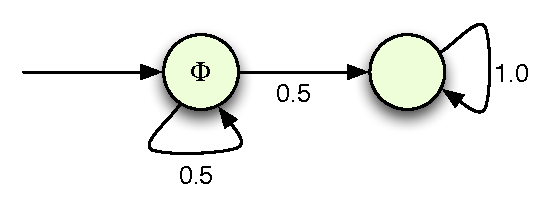
\includegraphics[scale=.85]{../GFX/Answer-A1-4b.pdf}
	\end{center}
	\caption{DTMC for question A1.4b}
	\label{fig:1a14b}
\end{figure}

\subsubsection*{A1.4c) Explaining why}
The CTL formula holds because there exists a path from $s_0$ where for the rest of time $s_0$ will be satisfied which is because it will loop forever. Where as the PCTL formula has probability and it is therefore unlikely that it will loop forever.

\subsubsection*{A1.4d) Feature of CTL}
The quantifier $E$ is required in order for the semantics of these formulae to be the same. Since there are probabilities involved there will aways be a chance that it will step out of the loop. Meanwhile in CTL there should just be a path that satisfies the specified property.

\section*{A2) Theoretical Problems}
\begin{figure}[H]
	\begin{center}
		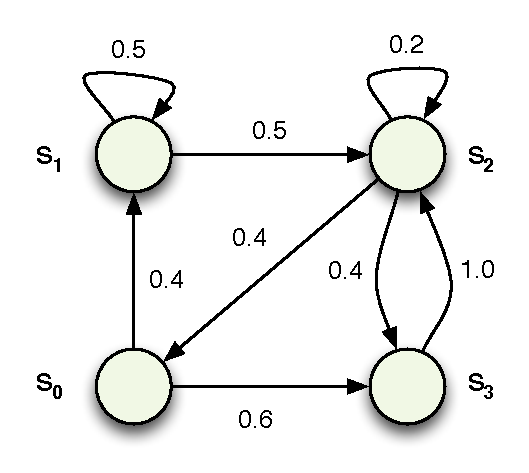
\includegraphics[scale=.85]{../GFX/ExerciseFigure1.pdf}
	\end{center}
	\caption{DTMC for questions A2.1 and A2.2}
	\label{fig:2a12}
\end{figure}

\subsection*{A2.1}
We have to consider the DTMC in Figure \ref{fig:2a12}, which is shown above and have initial state $s_0$.

\subsubsection*{A2.1a) Probability transition}
The initial distribution for the DTMC is as follows:
$$\iota_{init} = \left(1, 0, 0, 0\right)$$

The probability transition matrix for the DTMC is as follows:
$$\mathrm{\textbf{P}} = \left(
\begin{array}{c c c c}
	0 & 0.4 & 0 & 0.6\\
	0 & 0.5 & 0.5 & 0\\
	0.4 & 0 & 0.2 & 0.4\\
	0 & 0 & 1 & 0
\end{array}
\right)$$

\subsubsection*{A2.1b) Transient distribution}
The transient distribution, $\Theta$, up until the first three time steps is as follows:
\begin{center}
	\begin{tabular}{c c c c c c c c}
	& & & $s_0$ & $s_1$ & $s_2$ & $s_3$\\
	$\Theta_0$ & = & [ & 1.00 & 0.00 & 0.00 & 0.00 & ]\\
	$\Theta_1$ & = & [ & 0.00 & 0.40 & 0.00 & 0.60 & ]\\
	$\Theta_2$ & = & [ & 0.00 & 0.20 & 0.80 & 0.00 & ]\\
	$\Theta_3$ & = & [ & 0.32 & 0.10 & 0.26 & 0.32 & ]
	\end{tabular}
\end{center}

\subsubsection*{A2.1c) Steady state solution}
We have to calculate the steady state solution. First off, let's write down the equation matrix.
$$
	\left[
	\begin{matrix}
		P_1 & P_2 & P_3 & P_4
	\end{matrix}
	\right] \left[
	\begin{matrix}
		0 & 0.4 & 0 & 0.6\\
		0 & 0.5 & 0.5 & 0\\
		0.4 & 0 & 0.2 & 0.4\\
		0 & 0 & 1 & 0
	\end{matrix}
	\right] = \left[
	\begin{matrix}
		P_1 & P_2 & P_3 & P_4
	\end{matrix}
	\right]
$$
Now let's solve the equation.
\begin{description}
	\item[Step 1] Writing up the equations.
	$$\begin{array}{r c l c}
		P_1 & = & 0P_1 + 0P_2 + 0.4P_3 + 0P_4 & \Rightarrow\\
		P_1 & = & 0.4P_3\\
		\\
		P_2 & = & 0.4P_1 + 0.5P_2 + 0P_3 + 0P_3 & \Rightarrow\\
		P_2& = & 0.4P_1 + 0.5P_2\\
		\\
		P_3 & = & 0P_1 + 0.5P_2 + 0.2P_3 + P_4 & \Rightarrow\\
		P_3 & = & 0.5P_2 + 0.2P_3 + P_4\\
		\\
		P_4 & = & 0.6P_1 + 0P_2 + 0.4P_3 + 0P_4 & \Rightarrow\\
		P_4 & = & 0.6P_1 + 0.4P_3\\
		\\
		1 & = & P_1 + P_2 + P_3 + P_4
	\end{array}$$
	
	\item[Step 2] Reducing the equations.
	$$\begin{array}{r c l c}
		P_1 & = & 0.4P_3\\
		\\
		P_2 & = & 0.4P_1 + 0.5P_2 & \Rightarrow\\
		0.5P_2 & = & 0.4P_1 & \Rightarrow\\
		P_2 & = & 0.8P_1\\
		\\
		P_3 & = & 0.5P_2 + 0.2P_3 + P_4 & \Rightarrow\\
		0.8P_3 & = & 0.5P_2 + P_4 & \Rightarrow\\
		P_3 & = & 0.625P_2 + 1.25P_4\\
		\\
		P_4 & = & 0.6P_1 + 0.4P_3
	\end{array}$$
	
	\item[Step 3] Substituting $P_1$.
	$$\begin{array}{r c l c}
		P_2 & = & 0.8(0.4P_3) & \Rightarrow\\
		P_2 & = & 0.32P_3\\
		\\
		P_4 & = & 0.6(0.4P_3) + 0.4P_3 & \Rightarrow\\
		P_4 & = & 0.24P_3 + 0.4P_3 & \Rightarrow\\
		P_4 & = & 0.64P3\\
		\\
		1 & = & 0.4P_3 + P_2 + P_3 + P_4 & \Rightarrow\\
		1 & = & P_2 + 1.4P_3 + P_4
	\end{array}$$
	
	\item[Step 4] Substituting $P_2$.
	$$\begin{array}{r c l c}
		P_3 & = & 0.625(0.32P_3) + 1.25P_4 & \Rightarrow\\
		P_3 & = & 0.2P_3 + 1.25P_4 & \Rightarrow\\
		0.8P_3 & = & 1.25P_4 & \Rightarrow\\
		P_3 & = & 1.5625P_4\\
		\\
		1 & = & 0.32P_3 + 1.4P_3 + P_4 & \Rightarrow\\
		1 & = & 1.72P_3 + P_4
	\end{array}$$
	
	\item[Step 5] Calculating $P_3$.
	$$\begin{array}{r c l c}
		1 & = & 1.72P_3 + 0.64P_3 & \Rightarrow\\
		1 & = & 2.36P_4 & \Rightarrow\\
		P_3 & = & \frac{1}{2.36} & \Rightarrow\\
		P_3 & = & 0.42372881355 
	\end{array}$$
	
	\item[Step 5] Calculating $P_4$.
	$$\begin{array}{r c l c}
		1 & = & 1.72(1.5626P_4) + 1P_4 & \Rightarrow\\
		1 & = & 2.687672P_4 + 1P_4 & \Rightarrow\\
		1 & = & 3.687662P_4 & \Rightarrow\\
		P_4 & = & \frac{1}{3.687662} & \Rightarrow\\
		P_4 & = & 0.27117452738 
	\end{array}$$
	
	\item[Step 6] Calculating $P_1$.
	$$\begin{array}{r c l c}
		P_1 & = & 0.4P_3 & \Rightarrow\\
		P_1 & = & 0.4(0.42372881355) & \Rightarrow\\
		P_1 & = & 0.16949152542
	\end{array}$$
	
	\item[Step 7] Calculating $P_2$.
	$$\begin{array}{r c l c}
		P_2 & = & 0.8P_1 & \Rightarrow\\
		P_2 & = & 0.8(0.16949152542) & \Rightarrow\\
		P_2 & = & 0.13559322033
	\end{array}$$
\end{description}

So to sum up we have the following steady state probabilities for the DTMC:
$$\left[
	\begin{matrix}
		0.16949152542 & 0.13559322033 & 0.42372881355 & 0.27117452738
	\end{matrix}
\right]$$

\subsection*{A2.2}
The DTMC from Figure \ref{fig:2a12} encoded as a PRISM module:
\lstinputlisting[style=prismmodel,caption={PRISM module encoding the DTMC from Figure \ref{fig:2a12}.}]{../Code/A2.2.pm}

PRISM outputs the following transient distribution for the encoded DTMC:
\begin{lstlisting}[style=logoutput]
0:(0)=0.32000000000000006
1:(1)=0.1
2:(2)=0.26
3:(3)=0.32000000000000006
\end{lstlisting}
The above matches the calculated transient distribution from A2.1b.\\
\\
PRISM outputs the following steady state probabilities for the encoded DTMC:
\begin{lstlisting}[style=logoutput]
0:(0)=0.1694916167456058
1:(1)=0.1355931954330166
2:(2)=0.42372867450100926
3:(3)=0.2711865133203683
\end{lstlisting}
The above matches the calculated steady state solution from A2.1c.

\subsection*{A2.3}
\begin{figure}[H]
	\begin{center}
	\begin{tabular}{c c}
		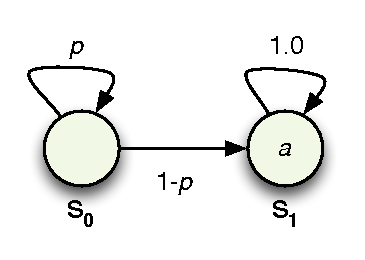
\includegraphics[scale=.85]{../GFX/ExerciseFigure2a.pdf} &
		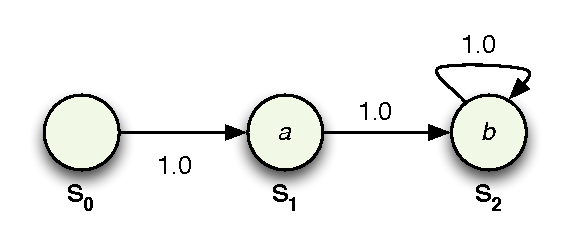
\includegraphics[scale=.85]{../GFX/ExerciseFigure2b.pdf}\\
		\textbf{\Large(a)} & \textbf{\Large(b)}
	\end{tabular}
	\end{center}
	\caption{DTMCs for question A2.3}
	\label{fig:2a3}
\end{figure}

We have to consider the DTMC in Figure \ref{fig:2a3}(a), which is shown above and have initial state $s_0$.

\subsubsection*{A2.3a) Values for $p$ which holds for $s_0 \models \mathbb{P}_{\geq \frac{1}{2}}(F^{\leq 2}\; a)$}
We have a maximum of two steps to reach $a$ with a probability of at least $\frac{1}{2}$. In other words we have to solve:
$$(1-p)^2 \geq \frac{1}{2} \quad | \quad 0 \leq p \leq 1$$

This gives:
$$0 \leq p \leq 0.292893$$

\subsubsection*{A2.3b) Expected number of time steps until $a$ holds in terms of $p$}
We have to calculate the \emph{Markov chain sojourn time}. We look at the probability of leaving the initial state $s_0$, thereby reaching $a$ for some amount of steps.

\begin{description}
	\item[Define $p_s$] The probability of staying in the same state, in this case $s_0$, is defined as:
	$$p_s = 1 - P(s_0, s_0)$$
	
	\item[Probability after one time step] The probability of staying in $s_0$ after one time step is:
	$$\mathrm{\textbf{Pr}}_{s_0}(N_{s_0}=1)=p_s$$
	
	\item[Probability after two time steps] The probability of staying in $s_0$ after two time steps is:
	$$\mathrm{\textbf{Pr}}_{s_0}(N_{s_0}=2)=(1-p_s) \cdot p_s$$
	
	\item[Probability after $n$ time steps] The probability of staying in $s_0$ after $n$ time steps is:
	$$\mathrm{\textbf{Pr}}_{s_0}(N_{s_0}=n)=(1-p_s)^{(n-1)} \cdot p_s$$
	
	\item[Rewriting] The probability of staying in $s_0$ after $n$ times steps can also be written as:
	$$\mathrm{\textbf{Pr}}_{s_0}(N_{s_0} \leq n) = \sum_{i=1}^{n} \mathrm{\textbf{Pr}}_{s_0}(N_{s_0} = i)  = 1 - (1-p_s)^n$$
	
	\item[Expected number of time steps spend in state $s_0$] Can be calculated using the formula below:
	$$\begin{array}{r c l}
	\mathrm{E}[N_{s_0}] & = & \sum_{i=1}^{n} \mathrm{\textbf{Pr}}_{s_0}(N_{s_0} = i)\cdot i\\[0.15cm]
	& = & \sum_{n=1}^{\infty} \mathrm{\textbf{Pr}}_{s_0}(N_{s_0} \geq n)\\[0.15cm]
	& = & \sum_{n=1}^{\infty} (1-p_s)^{n-1}\\[0.15cm]
	& = & \frac{1}{p_s}
	\end{array}$$
	
	\item[Replacing $p_s$] We have to state the expected number of time steps in terms of $p$, therefore we start by replacing $p_s$:
	$$\mathrm{E}[N_{s_0}] = \frac{1}{1 - P(s_0,s_0)}$$
	We then replace $P(s_0,s_0)$:
	$$\mathrm{E}[N_{s_0}] = \frac{1}{1 - p}$$
\end{description}

\subsubsection*{A2.3c) DTMC modification}
We have to modify Figure \ref{fig:2a3}(b), without increasing the number of states, so that the following holds:
$$s_0 \models \mathbb{P}_{\geq \frac{1}{2}}(\diamondsuit^{=5}\; a)$$
$$s_1 \models \mathbb{P}_{\geq \frac{1}{2}}(\diamondsuit^{=10}\; b)$$

\begin{description}
	\item[Reaching $s_1$ from $s_0$] To do this in five time steps we have to calculate the probability of $s_0$ going to $s_0$, while ensuring that on average 5 time time steps will be enough to reach $s_1$. We calculate it the following way:
	$$5 = \frac{1}{1-p} \Rightarrow \ldots \Rightarrow p = \frac{4}{5}$$
	So to ensure that on average 5 time steps will be required to go from $s_0$ to $s_1$ we must add the following to the DTMC:
	$$s_0 \xrightarrow{0.8} s_0$$
	
	\item[Reaching $s_2$ from $s_1$] To do this in 10 time steps we have to calculate the probability of $s_1$ going to $s_1$, while ensuring that on average 10 time steps will be enough to reach $s_2$. We calculate it the following way:
	$$10 = \frac{1}{1-p} \Rightarrow \ldots \Rightarrow p = \frac{9}{10}$$
	So to ensure that on average 10 time steps will be required to go from $s_1$ to $s_2$ we must add the following to the DTMC:
	$$s_1 \xrightarrow{0.9} s_1$$
	
	\item[The modified DTMC] Below is the modified DTMC:
	\begin{figure}[H]
		\begin{center}
		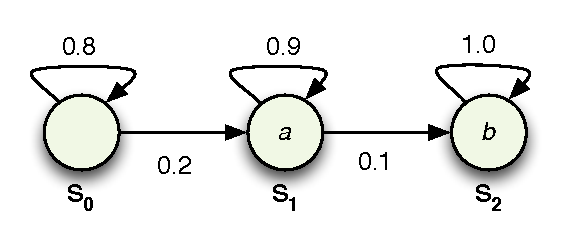
\includegraphics[scale=.85]{../GFX/Answer-A2-3c.pdf}
		\end{center}
		\caption{Modified version of the DTMC from Figure \ref{fig:2a3}.}
	\end{figure}
\end{description}

\subsection*{A2.4}
\begin{figure}[H]
	\begin{center}
		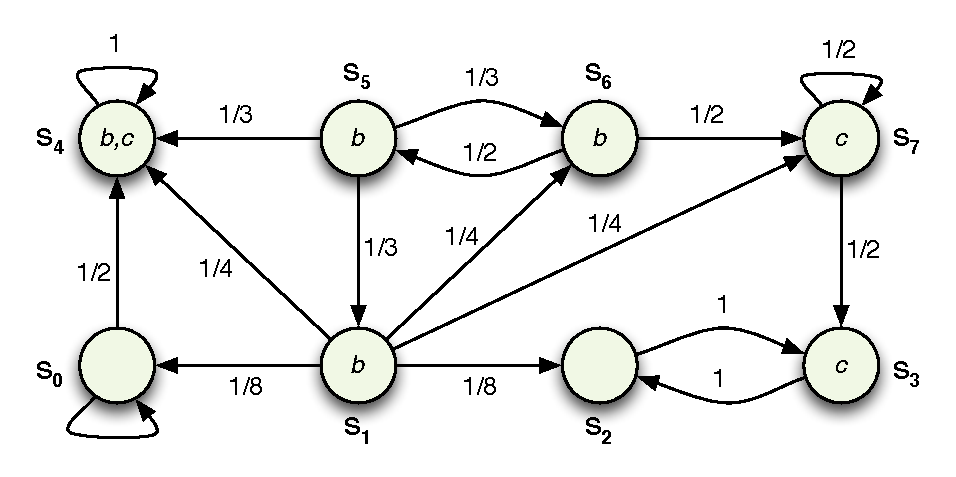
\includegraphics[scale=.85]{../GFX/ExerciseFigure3.pdf}
	\end{center}
	\caption{DTMC for question A2.4}
	\label{fig:2a4}
\end{figure}

We have to consider the DTMC in Figure \ref{fig:2a4}, which we will call $\mathcal{M} = \left(S, \mathbf{P}, s_1, AP, L\right)$, where $AP = \{b,c\}$. The initial state is $s_1$ and the labels are shown on the states.

\subsubsection*{2A.4a) Determine which states satisfy $\mathbb{P}_{\geq\frac{17}{19}}(b\;U\;c)$}
The set of satisfying states is:
$$\{s_3, s_4, s_6, s_7\}$$

\subsubsection*{2A.4b) Determine which states satisfy $\mathbb{P}_{\geq\frac{1}{2}}\left(X\;\mathbb{P}_{>\frac{1}{3}}\left( \left(b \vee c \right) U^{\leq 2} \left( b \wedge c \right) \right) \right)$}
The set of satisfying states is:
$$\{s_0, s_4, s_6\}$$

\chapter*{Part B: Intermediate Problems}
\section*{B1) Practical Problems}
\subsection*{Lottery scheduler}
In this part we will model a Lottery Scheduler (found in the \emph{LotteryScheduler.pm} file). In Lottery Scheduling each task is assigned a number of tickets. When the scheduler has to decide which task to execute, the scheduler selects a ticket under a uniform distribution, and the task owning the ticket is allowed to execute. Our Lottery Scheduler is \emph{pre-emptive} which means that a task can only execute for a certain amount of time before being interrupted. In our scheduler the amount of time is one time unit.  Our Lottery Scheduler has three clients with one task each. Each task has a single ticket. We have modeled the tickets as a single variable in the scheduler module. The variable called \emph{ticket} has a range of 0 to 3 and it is initialized as 0. The serving of the jobs is as follows: Whenever a task is in the scheduler it is allowed to execute for one time unit given that the ticket has a value equal to the client's number. After the job has executed for one time unit the variable ticket is assigned to 0. The exciting part is assigning the value of the ticket.

\begin{lstlisting}[style=prismmodel]
  [] ticket=0 -> 0.333333333333333333333333:(ticket'=1) + 0.333333333333333333333333:(ticket'=2) + 0.333333333333333333333333:(ticket'=3);
  [] job1=false & ticket=1 -> 0.5:(ticket'=2) + 0.5:(ticket'=3);
  [] job2=false & ticket=2 -> 0.5:(ticket'=1) + 0.5:(ticket'=3);
  [] job3=false & ticket=3 -> 0.5:(ticket'=1) + 0.5:(ticket'=2);
\end{lstlisting}
Whenever the ticket is 0 there should be an equal probability of choosing one of the three jobs. But however it is possible that not all clients have a job in the scheduler which is why it is necessary with the other three commands. Here the value of the ticket is assigned with equal probability 0.5 since there are only two jobs in the scheduler.

\subsubsection*{Executing time for $client_1$}
We are interested in the time taken for the first task from $client_1$ to complete. In order to do this we introduce a new module called \emph{Monitor}. Monitor has only one variable called finished which is a boolean value. It is initialized as false. When the finish1 command is executed meaning the first job from $client_1$ has completed the finished variable will be set to true. For subsequent actions it remains in this state.\\
We write a PCTL formula using the '$\mathbb{P}_{=?}$' syntax expressing that the first task from $client_1$ completes within in $t$ time units. $t$ is defined as an integer constant without a value. We will use the experimentation feature of PRISM to plot a graph of this probability for $0 \leq t \leq 20$.\\
The PCTL formula: $\mathbb{P}_{=?}(\diamondsuit^{\leq t} finished=true)$
\begin{figure}[H]
	\centering
	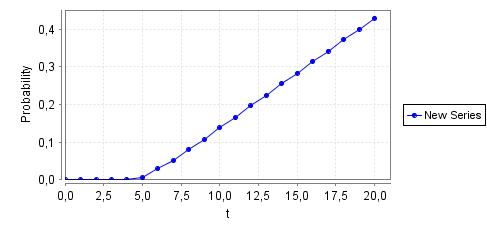
\includegraphics[scale=0.75]{../GFX/B1-1c.png}
	\caption{A graph plotting the probability for $0 \leq t \leq 20$ with one time unit for $\mathbb{P}_{=?}(\diamondsuit^{\leq t} finished=true)$}
\end{figure}

\subsubsection*{Starvation}
We are interested in finding out whether it is possible for our lottery scheduler to suffer from starvation. In order to determine this we specify some PCTL formula which we will use PRISM to verify. The PCTL formulae states that whenever task1, task2 or task3 is greater than zero there must be a probability of greater than or equal to 1 that task1, task2 or task3 will eventually be zero. This means that whenever a job is created it will be served until it is finished.
\begin{center}
$(task1 > 0) \Rightarrow \mathbb{P}_{\geq 1}(F(task1 = 0))$\\
$(task2 > 0) \Rightarrow \mathbb{P}_{\geq 1}(F(task2 = 0))$\\
$(task3 > 0) \Rightarrow \mathbb{P}_{\geq 1} (F(task3 = 0))$
\end{center}
These properties have been verified by PRISM so it is not possible in our model that our lottery scheduler will suffer from starvation.

\subsubsection*{Two time units modification}
We wish to modify our allowed time for execution for each task so that is two time units (found in the file \emph{LS-2units.pm}). We do this by defining an integer variable called \emph{time} with a range between 0 and 2. Whenever the variable ticket is 0 then it will assign ticket to a value according to each client with an equal probability as before but now it will also set the variable time to 2. The guards for the serve commands now have an additional condition which is that time must be greater than 0. Meanwhile whenever time is 0 and ticket is above 0 ticket will be reset to 0 so a new job can be served. Furthermore whenever finish for a job is activated it will reset time to 0. The interesting part is how this affects the time taken to complete a task from $client_1$. We will do the same as before and make a graph.
\begin{figure}[H]
	\centering
	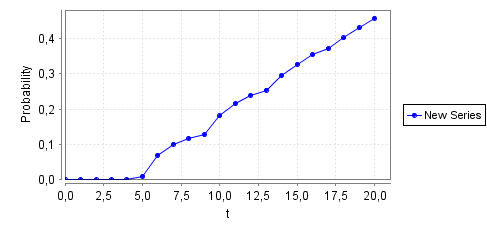
\includegraphics[scale=0.75]{../GFX/B1-1e.png}
	\caption{A graph plotting the proprobability for $0 \leq t \leq 20$ with two time units}
\end{figure}
As we can see by the graph it does not affect the total probability much but the graph has larger spikes in probability because the time unit is now increased by 1.

\subsection*{Priority Lottery Scheduler}
Instead of assigning the same number of tickets to each task we now give varying priority to different tasks by assigning them different numbers of tickets. This variant of the lottery scheduler can be found in the file \emph{PLS.pm}. We will approximate a Shortest Remaining Time scheduler by using this kind of lottery scheduling. This means that small tasks will be assigned more tickets than a large task. We have done this approximation by creating three integer variables with range from 0 to 5 and they are initialized as 0. These three variables are called ticket1, ticket2 and ticket3 - one for each client. When a client creates a job the client must not have a job in the scheduler already or the client's corresponding ticket may not be any other value than 0. This is because the ticket belonging to the client will get its value by subtracting the length of its job from the maximum length of a job (5). Meaning that a job of length 5 will be assigned a ticket value of 0. When the jobs in the scheduler are finished their ticket values will be reset to 0. The serving of the jobs have a guard that specifies that its ticket value must be greater or equal to the other tickets in order to be served.

\subsubsection*{Time taken and Starvation}
We wish to find out how this affects the time taken to complete a task from $client_1$. We will once again plot a graph for the probability.
\begin{figure}[H]
	\centering
	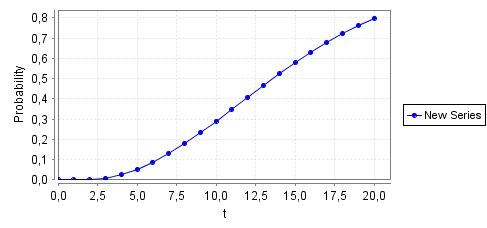
\includegraphics[scale=0.75]{../GFX/B1-2b.png}
	\caption{A graph plotting the probability for $0 \leq t \leq 20$ with priorities}
\end{figure}
As we can see by the graph adding priorities will affect the time taken to complete a task from $client_1$. It now has a higher probability of finishing a job within 20 time steps because all the small jobs will be served first by the scheduler.
\\Also we would like to find out if starvation is possible in our model. We therefore use the following PCTL formula to verify the properties in PRISM.
\begin{center}
$(task1 > 0) \Rightarrow \mathbb{P}_{\geq 1}(F(task1 = 0))$\\
$(task2 > 0) \Rightarrow \mathbb{P}_{\geq 1}(F(task2 = 0))$\\
$(task3 > 0) \Rightarrow \mathbb{P}_{\geq 1} (F(task3 = 0))$
\end{center}
These properties have been verified by PRISM meaning that a job will always complete but it is worth noting that it can take a job of length 5 a long time to complete if the other clients keep creating shorter jobs.

\subsubsection*{Investigation of the model}
We want to increase the number of clients in our model until we reach the maximum for which PRISM can still build and solve the underlying DTMC. We do this by just incrementing and building till PRISM cannot build anymore. This gives us a maximum of 8 clients. It takes a time to build the model. With trying to build with 9 clients PRISM shut down with no errors.\\
In general having a scheduler that uses priority based scheduling or a shortest time based scheduling will make the scheduler vulnerable to denial of service attack. Because in our model  if a client tries to perform long jobs but all the other clients generate very short jobs. The short jobs will move ahead of the queue and the long jobs will never be served if there always will be generated more short jobs. It would be desirable to express denial of service as a PCTL property but this is not possible for our model. This is because in our model the job will always complete it is just a question of time. We cannot express a PCTL property that will create a job every time the old short job finished.

\section*{B2) Theoretical Problems}
\subsection*{Modyfing the step-bounded until operator}
A step bounded formula $\Phi_1\;U^{\leqslant n}\;\Phi_2$ satisfies the needs for making assumptions regarding a specific type of interval, $I = [0, n]$, we would like to introduce a more generalized operator in the form of:
$$\Phi_1\;U^{I}\;\Phi_2 \quad | \quad I \in \left\{\;[n,n'],\;[n, n'[,\;]n, n],\;]n, n'[\;\right\} \quad | \quad 0 \leq x \leq y$$

\subsubsection*{Adapting PCTL}
To make this new operator possible using only PCTL, we have to synthesize the new operator using our currently available operators. We're not allowed to simply modify the current until operator to satisfy more cases, such a modification could be like:
$$\Phi_1\;U^{[n, \infty[}\;\Phi_2 = \Phi_1\;U^{\geqslant n}\;\Phi_2$$
Which would state that after $n$ steps $\Phi_1$ should hold up until at some point where $\Phi_2$ would hold.\\
\\
There are 10 important cases of how the intervals can be constructed, let's look at them case by case:
\begin{description}
	\item[Case 1:] $[0, 0]$\\
	This is the same as skipping the left part of the operator:
	$$\Phi_2$$

	\item[Case 2:] $[0, n]$\\
	This is the same as the current bounded until operator:
	$$\Phi_1\;U^{\leqslant n}\;\Phi_2$$
	
	\item[Case 3:] $[0,n[$ where $0 < n$\\
	This is the same as an interval of $[0, n-1]$, therefore it will either match \textbf{Case 1} or \textbf{Case 2}.
	
	\item[Case 4:] $[0, \infty[$\\
	This is the same as the unbounded until operator, so we would write this as:
	$$\Phi_1\;U\;\Phi_2$$
	
	\item[Case 5:] $[n, \infty[$\\
	Not possible as you would have to set a restriction of when the left part of the operator should apply. If we were to have a \emph{Time Step} property, this would be possible.\\
	Let's define a time step property, first we need a symbol for it:
	$$\mathbb{T}$$
	Then we need a syntax:
	$$\mathbb{T}^{\leqslant n} = \left\{
		\begin{array}{c l}
			\text{true} & \text{if } n \leq \text{amount of time steps passed}\\
			\text{false} & \text{if } n > \text{amount of time steps passed}
		\end{array}
	\right.$$
	$$\mathbb{T}^{\geqslant n} = \left\{
		\begin{array}{c l}
			\text{true} & \text{if } n \geq \text{amount of time steps passed}\\
			\text{false} & \text{if } n < \text{amount of time steps passed}
		\end{array}
	\right.$$
	Formally the syntax states that if the expression for $n$ satisfies for the amount of time steps passed then it returns \textbf{true}, otherwise it will return \textbf{false}.\\
	\\
	We can use this new property to specify a starting point for our modified until operator. Using the new syntax we can properly write out the adapted PCTL for the case:
	$$\mathbb{T}^{\geqslant n} \wedge \mathbb{P}_{=1}\left(\Phi_1\;U\;\Phi_2\right)$$
	
	\item[Case 6:] $]0, \infty[$\\
	This can be rewritten to $[1, \infty[$, which can be interpreted as $[n, \infty[$. See Case 5.
	
	\item[Case 7:] $]n, \infty[$ where $0 < n$\\
	This can be rewritten to $[n+1, \infty[$, which is covered by Case 5.
	
	\item[Case 8:] $[n, n']$\\
	We have to make use of our time step property again. This time there's both a limitation of when to start and a limitation of when to end.
	$$\mathbb{T}^{\geqslant n} \wedge \mathbb{P}_{=1}\left(\Phi_1\;U^{\leqslant n'}\;\Phi_2\right)$$
	
	\item[Case 9:] $]n, n']$ where $n < n'$\\
	This can be rewritten to $[n+1, n']$
	
	\item[Case 10:] $]n, n'[$ where $n < n + 1 < n'$\\
	This can be rewritten to $[n+1, n'-1]$.
\end{description}

So with the introduction of our time step operator, we can model the modified version of the until operator in PCTL.

\subsubsection*{Adapting the model checking algorithm}
We cant just introduce a new property to PCTl by specifying its syntax and how it works, we must also state how the model checking algorithm should use this new property.\\
\\
Basically the new time step property should be treated as \text{true} and the atomic propositions are being treated. In general the way the model checking is performed wouldn't have had any major changes, though it is important that the algorithm keeps track of time steps.

\subsection*{Bisimulation relations}
\begin{figure}[H]
	\begin{center}
		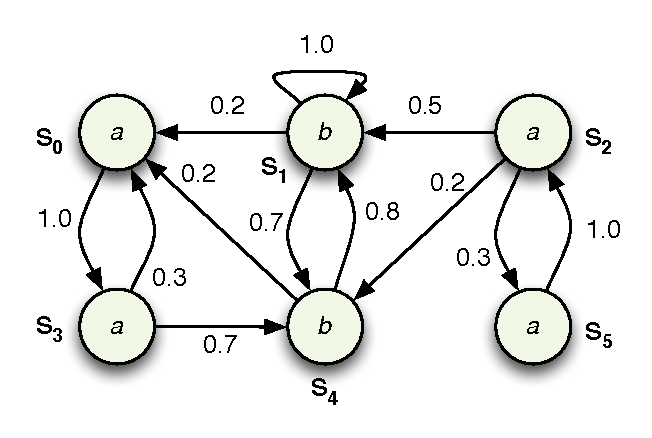
\includegraphics[scale=.85]{../GFX/ExerciseFigure4.pdf}
	\end{center}
	\caption{DTMC for question B2.2}
	\label{fig:b22}
\end{figure}

We have to consider the DTMC in Figure \ref{fig:b22}, which we will call $\mathcal{M} = \left(S, \mathbf{P}, s_0, AP, L\right)$, where $AP = \{a,b\}$. The initial state is $s_0$ and the labels are shown on the states.
We write down the coarsest probabilistic bisimulation relation between the states of $\mathcal{M}$: $R \subseteq S \times S$.
$$R = \left\{\begin{array}{c}
(s_0, s_0), (s_0,s_5),(s_1,s_1), (s_1,s_4),(s_2,s_2),(s_2,s_3),\\(s_3,s_2),(s_3,s_3),(s_4,s_4),(s_4,s_1),(s_5,s_5),(s_5,s_0)
\end{array}\right\}$$

This relation is a probabilistic bisimulation. This can be seen as follows. States $s_0$ and $s_5$ can move to a state with label $a$ with probability 1. States $s_1$ and $s_4$ can both move to a state with label $b$ with probability 0.8 and to a state with label $a$ with probability 0.2. States $s_2$ and $s_3$ can move to a state with label $b$ with probability 0.7 and to a state with label $a$ with probability 0.3.\\
\\
We have constructed the bisimulation quotient $\mathcal{M} / \sim$ of $\mathcal{M}$. This can be seen in the figure below.
\begin{figure}[H]
	\begin{center}
		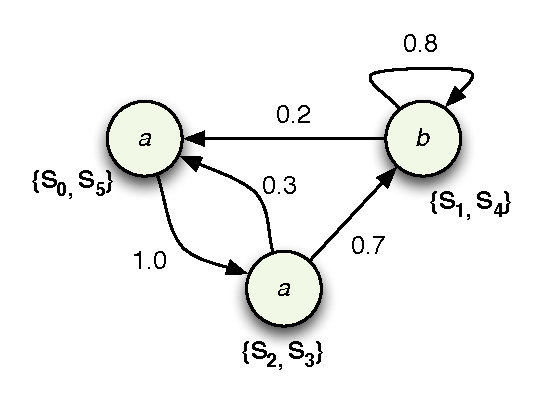
\includegraphics[scale=.85]{../GFX/Answer-B2-2b.pdf}
	\end{center}
	\caption{Bisimulation quotient $\mathcal{M} / \sim$ of $\mathcal{M}$.}
	\label{fig:b22b}
\end{figure}

The steady state probabilities of $\mathcal{M}$ are:
$$\begin{array}{l c l}
	s_0 & = & 0.06761927768284443\\
	s_1 & = & 0.3840264466025563\\
	s_2 & = & 0.1097219095822044\\
	s_3 & = & 0.06761930771595279\\
	s_4 & = & 0.3380965125386377\\
	s_5 & = & 0.03291654587780441
\end{array}$$

The steady state probabilities of $\mathcal{M} / \sim$ are:
$$\begin{array}{l c l}
	s'_0 & = & 0.18181825070431698\\
	s'_1 & = & 0.6363636180884598\\
	s'_2 & = & 0.1818181312072233
\end{array}$$
The steady state probabilities for $\mathcal{M}$ relates to the steady state probabilities of $\mathcal{M} / \sim$. $s_1, s_4$ which corresponds to $s'_1$ are the highest.

\subsubsection*{Relabeling}
If we would could choose a labeling function $L$ for the DTMC $\mathcal{M}$ that would help make the coarsest possible probabilistic bisimulation, then the function would be:
$$L = \left\{\begin{array}{l c r}
s_0 & = & a\\
s_1 & = & a\\
s_2 & = & a\\
s_3 & = & a\\
s_4 & = & a\\
s_5 & = & a
\end{array}\right\}$$

This would result in the coarsest possible probabilistic bisimulation being:
$$R = \left\{\begin{array}{c}
(s_0, s_0),(s_0,s_1),(s_0,s_2),(s_0,s_3),(s_0,s_5),(s_0,s_5),\\
(s_1, s_0),(s_1,s_1),(s_1,s_2),(s_1,s_3),(s_1,s_5),(s_1,s_5),\\
(s_2, s_0),(s_2,s_1),(s_2,s_2),(s_2,s_3),(s_2,s_5),(s_2,s_5),\\
(s_3, s_0),(s_3,s_1),(s_3,s_2),(s_3,s_3),(s_3,s_5),(s_3,s_5),\\
(s_4, s_0),(s_4,s_1),(s_4,s_2),(s_4,s_3),(s_4,s_5),(s_4,s_5),\\
(s_5, s_0),(s_5,s_1),(s_5,s_2),(s_5,s_3),(s_5,s_5),(s_5,s_5)
\end{array}\right\}$$
All states have equal probability of 1 of reaching a state with label $a$. 

\subsubsection*{Lumpability}
Probabilistic bisumilation has an equivalent formulation called \emph{lumpability}. A partitioning of the state space os a DTMC (i.e. a labelling function $L$ such that $|L(s)| = 1$ for all $s$) is said to be lumpable if for all pairs of states $s_1,s_2 \in S$ such that $L(s_1) = L(s_2)$, and all atomic propositions $a \in AP$:
$$\sum_{s' \in L^{-1}(a)} \mathbf{P}(s_1,s') = \sum_{s' \in L^{-1}(a)} \mathbf{P}(s_2,s')$$

It can be proven that probabilistic bisimulation implies lumpability. For a pair of states $s_1, s_2 \in \mathcal{R}$, the probabilistic bisimulation, the following must be true:
\begin{enumerate}
	\item $L(s_1) = L(s_2)$
	\item $\mathbf{P}(s_1, T) = \mathbf{P}(s_2, T)$ for each equivalence class $T \in S / \mathcal{R}$
\end{enumerate}

Both probabilistic bisimulation and lumpability requires that the probability of moving by a single transition to some equivalence class is equal. Further probabilistic bisimulation requires that the labeling for the states are equal. As stated earlier the labeling function can be used for partitioning the state space. Therefore probabilistic bisimulation is a specific case of lumpability, which means that probabilistic bisimulation implies lumpability.\\
\\
If we wanted to distinguish between the two states of a lumpable partition using PCTL*, assuming the same labeling function has been used for both instances, then we will be having a pretty hard time. There are severals reason for that:
\begin{enumerate}
	\item It's not possible to distinguish the states by their label. It's a requirement that for two states to be in a lumpable partition, their labeling must be equal.
	\item It's not possible to distinguish the states by requiring the next state to be of a specific label. For two states to be in a lumpable parition, the probability of reaching a state with a specific label must be the same for both states, therefore you cannot use a PCTL* formula like $s \wedge \mathbb{P}_{=1}(\bigcirc \; a)$ to distinguish between the states, as the formula has to be true for both $s_1$ and $s_2$.
\end{enumerate}


\chapter*{Part C: Advanced Problems}
\section*{Practical Problems}
In this part we wish to extend our Priority Lottery Scheduler from part B1, where there are multiple servers. This means that we have to seperate the functionality of the scheduler from the execution of the tasks which previously have been combined in the module Scheduler. The scheduler has to decide the order of which the tasks execute and which server executes them. We will modify our lottery scheduler to model a system with two servers. In the following subsections we will describe how the scheduler chooses the order of executing tasks and and which server executes them in different scenarios. For each scenario we will investigate the relative responsiveness.

\subsection*{Probabilistically choice}
We have extended the priority lottery scheduler so that it chooses between the two servers with an equal probability. This extension can be found in the file \emph{PLS-2serversP.pm}. This extension has been done by making two modules called \emph{server1} and \emph{server2}. The scheduler is extended with new commands that will synchronise with either server1 or server2 which will be determined by the variable \emph{useserver}. Whenever useserver is 0 then it will be assigned to 1 with probability 0.5 and assigned to 2 with probability 0.5. The value 1 will cause the server1 to be used and likewise for server2. The scheduler is responsible for the priority of the tasks which will be used to determine which job will be served. The priority of the task are assigned to approximate a Shortest Remaining Time scheduler. The more ticket a job has the higher priority the job has. The scheduler module and the server modules synchronize over commands that specify that the task must have a high priority to be served and the specific server must be chosen by the useserver variable. The servers will use a variable changed by the synchronized commands with the scheduler to specify what job should be served and serve them by using the corresponding serve commands for the job. We now have to investigate how the probability of finishing the first task from $client_1$ evolve over time. We use PRISM to make an experiment with the following PCTL property:
$$\mathbb{P}_{=?}(\diamondsuit^{\leq t} finished=true)$$
Recall from earlier in the report that finished is a variable that will be assigned to true when the finish1 command is triggered. By using this PCTL property we have created a graph for $0 \leq t \leq 200$.
\begin{figure}[H]
	\begin{center}
		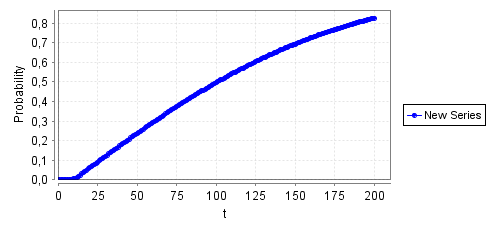
\includegraphics[scale=0.75]{../GFX/C1.png}
	\end{center}
	\caption{Graph for 2 servers with probabilistically choice}
\end{figure}
We can see by the graph how the probability of the first job from $client_1$ grows over time. At time step 200 it will have a probability of 0.8 of being finished which is quite high considering there are 84231 reachable states in the model.

Also we would like to find out if starvation is possible in our model. We therefore use the following PCTL formula to verify the properties in PRISM.
\begin{center}
$(task1 > 0) \Rightarrow \mathbb{P}_{\geq 1}(\diamondsuit(task1 = 0))$\\
$(task2 > 0) \Rightarrow \mathbb{P}_{\geq 1}(\diamondsuit(task2 = 0))$\\
$(task3 > 0) \Rightarrow \mathbb{P}_{\geq 1}(\diamondsuit(task3 = 0))$
\end{center}
These properties have been verified by PRISM meaning that a job will always complete.

\subsection*{High priority tasks}
We have extended the priority lottery scheduler so that one server is reserved for high priority tasks. This extension can be found in the file \emph{PLS-2servers-Priority.pm}. This extension also has two modules called server1 and server2, where server1 is reserved for high priority tasks. We use the notion that a task has high priority when it has 3 or more tickets. A task has at most 4 tickets. Server1 will only serve jobs with 3 or more tickets and server2 will just serve the tasks currently in the scheduler with the highest priority as before. This means that we no longer need a variable to keep track of what server to use next. It will just choose server1 if the task has 3 or more tickets. Nothing else has been changed from the previous extension with probabilistic choice. 
\\
We want to investigate how the probability of finishing the first task from $client_1$ evolve over time. We use PRISM to make an experiment with the same PCTL property as before.
$$\mathbb{P}_{=?}(\diamondsuit^{\leq t} finished=true)$$
By using this PCTL property we have created a graph for $0 \leq t \leq 200$. 337
\begin{figure}[H]
	\begin{center}
		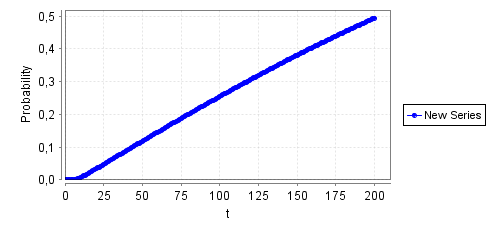
\includegraphics[scale=0.75]{../GFX/C2.png}
	\end{center}
	\caption{Graph for 2 servers with one server reserved for high priority tasks}
\end{figure}
We can see by the graph how the probability of finishing the first job from $client_1$ grows over time. At time step 200 it will have a probability of being finished. In a model with 131114 reachable states this is again quite high. It would be desirable to compare the two extensions to each other but this is difficult because of the big difference in reachable states. But the extensions however will never suffer from starvation and have a sensible probability of finishing jobs fast.
\\Again we would like to find out if starvation is possible in our extended model. We therefore use PRISM to verify the following PCTL properties.
\begin{center}
$(task1 > 0) \Rightarrow \mathbb{P}_{\geq 1}(\diamondsuit(task1 = 0))$\\
$(task2 > 0) \Rightarrow \mathbb{P}_{\geq 1}(\diamondsuit(task2 = 0))$\\
$(task3 > 0) \Rightarrow \mathbb{P}_{\geq 1}(\diamondsuit(task3 = 0))$
\end{center}
These properties have been verified by PRISM meaning that a job will always complete.

\end{document}
